\emph{Como producto del trabajo presentado en este capítulo surgió el artículo publicado en ``Pattern Recognition Letters'', volume 138, titulado ``$\tau$-SS3: A text classifier with dynamic n-grams for early risk detection over text streams''.}\footnote{\url{https://doi.org/10.1016/j.patrec.2020.07.001}}

\

El presente capítulo tiene como principal objetivo extender y complementar el trabajo presentado en el capítulo anterior, por lo que, a diferencia de este último, aquí no se hará un análisis cualitativo, o demasiado detallado, de los resultados obtenidos, en su lugar, el foco se pondrá en introducir una posible mejora del modelo original y no puntualmente en las tareas utilizadas para evaluarlo. Por este motivo, el rol de la experimentación en este capítulo se limitará, principalmente, a brindar un soporte empírico sobre el cual cuantificar la efectividad de la mejora propuesta.

\section{Introducción}


En el capítulo anterior se introdujo el nuevo modelo y se lo evaluó en el contexto de una tarea de detección de riesgos específica.
En particular, el modelo fue evaluado en la tarea piloto eRisk 2017 de detección anticipada de depresión, obteniendo resultados alentadores al superar a los otros modelos a pesar de su simpleza y transparencia.
Sin embargo, el modelo propuesto procesa a cada oración de la entrada utilizando, en esencia, un enfoque de \emph{bolsa de palabras} lo que, como se abordó en la \autoref{sec:tipo-termino} del \autoref{cap3}, provoca que la noción de orden entre las palabras se pierda.
% Sin embargo, nuestro modelo, SS3, en esencia procesa cada oración del stream de entrada utilizando una representación de bolsa de palabras (bag-of-words).
Esta característica lleva a que SS3 no tenga la capacidad de capturar secuencias de palabras importantes, como por ejemplo podría haber sido la secuencia ``kill myself'' en la \autoref{fig:subject9579_descriptive_c} del capítulo anterior, en donde sólo ``myself'' fue considerado por SS3 ---probablemente al ser ``myself'' una palabra de autorreferencia.
Esta incapacidad de capturar secuencias importantes podría afectar negativamente el rendimiento de la clasificación, como se puede intuir a partir del sencillo ejemplo mostrado en la \autoref{fig:ss3-example}.
Además, dado que las palabras individuales son menos informativas de lo que pueden llegar a ser ciertas secuencias de palabras, el uso de bolsa de palabras también reduce el poder descriptivo de las explicaciones visuales dadas por el modelo.
% However, at its core, SS3 processes each sentence from the input stream using a bag-of-word model. This leads to SS3 lacking the ability to capture important word sequences which could negatively affect the classification performance. Additionally, since single words are less informative than word sequences, this bag-of-word model reduces the descriptiveness of SS3's visual explanations.

\begin{figure*}[t!]
    \centering
    \centerline{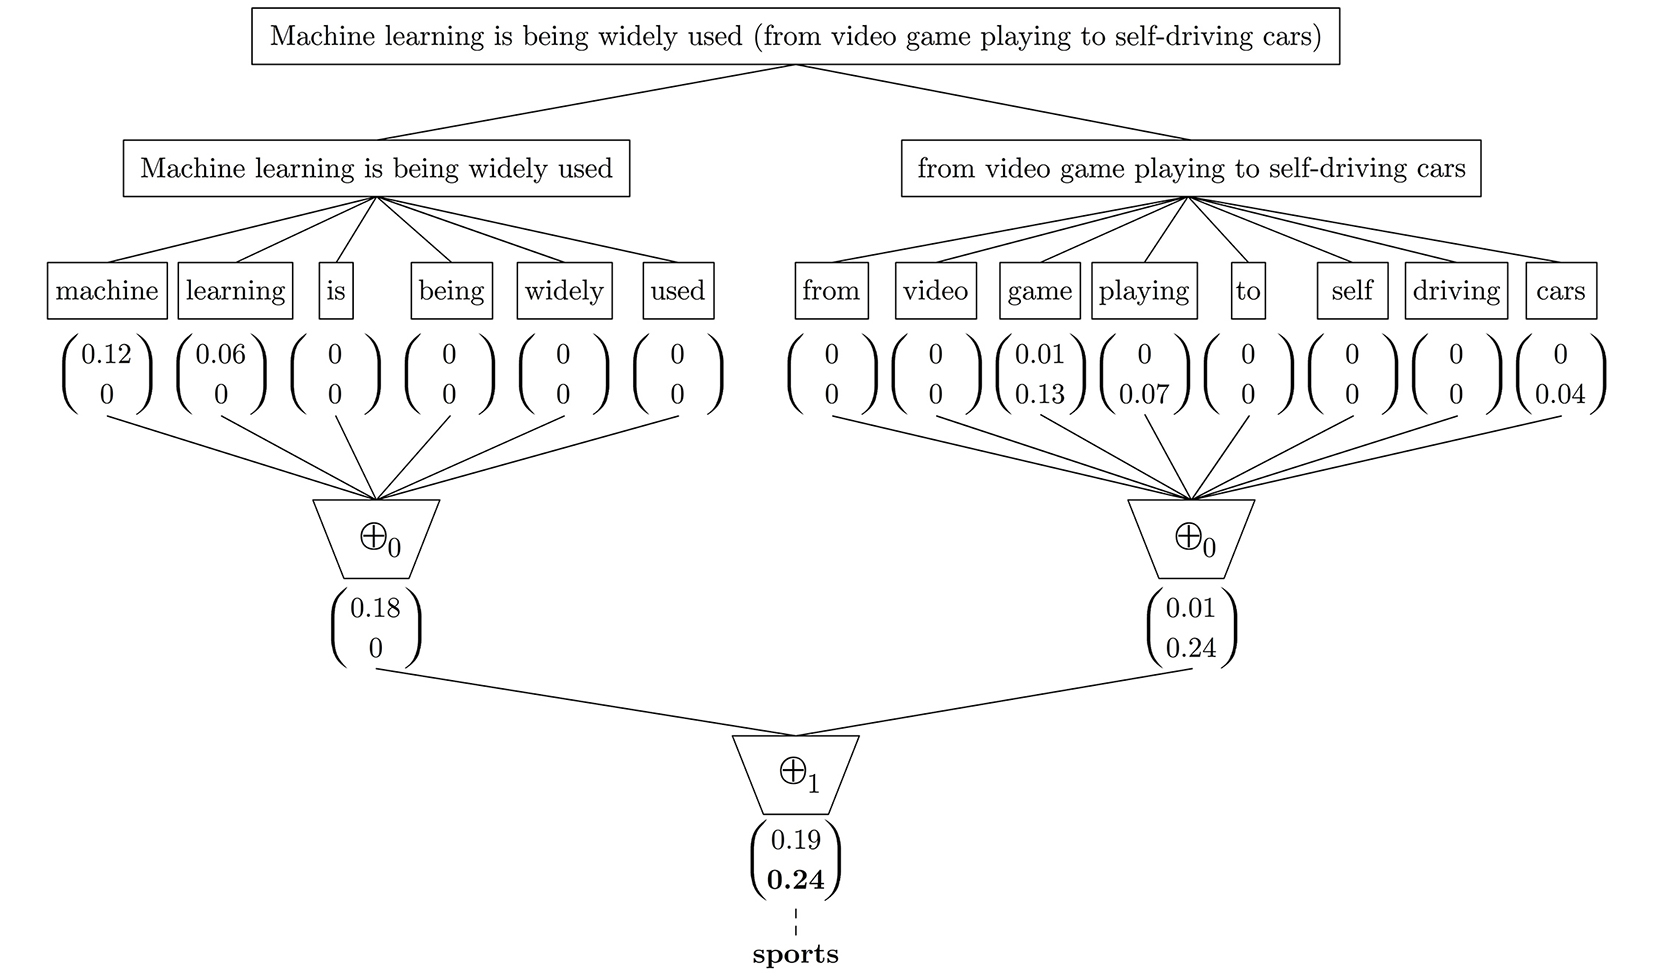
\includegraphics[width=190mm]{images/ss3-machine-learning}}
    \caption{
    Ejemplo de clasificación para las clases \emph{technology} y \emph{sports}.
    En este ejemplo, SS3 clasificó de forma incorrecta la temática del documento como \emph{sports}, ya que no puede capturar secuencias importantes para \emph{technology} como ser \emph{``machine learning''} o \emph{``video game''}.
    Esto se debe a que cada oración fue procesada como una bolsa de palabras.}
    % Classification example for categories \emph{technology} and \emph{sports}. In this example, SS3 misclassified the document's topic as $sports$ since it failed to capture important sequences for \emph{technology} like \emph{``machine learning''} or \emph{``video game''}. This was due to each sentence being processed as a bag of words.}
    \label{fig:ss3-example}
\end{figure*}

Una de las formas habituales para intentar mitigar algunas de las limitaciones de la representación de bolsa de palabras es identificar a los términos con n-gramas de palabras. De esta forma, el modelo mantiene, en cada término, alguna noción local del orden de las palabras de la entrada original.
% Las debilidades de las representaciones de bolsa de palabras son bien conocidas en el campo de clasificación de documentos tradicional, en el que generalmente se usan n-gramas de palabras para intentar remediarlas.
Desafortunadamente, cuando la entrada es una secuencia, en nuestro caso un flujo virtualmente infinito de texto, el uso de los n-gramas de palabras no es trivial, ya que, idealmente, los sistemas tienen que aprender a identificar dinámicamente qué n-gramas son los importantes ``sobre la marcha''.
% The weaknesses of bag-of-words representations are well-known in the standard document classification field, in which word n-grams are usually used to overcome them.
% Unfortunately, when dealing with text streams, using word n-grams is not a trivial task since the system has to dynamically identify, create and learn which n-grams are important ``on the fly''.
En este capítulo introducimos una generalización de SS3, llamada $\tau$-SS3, que expande su definición original permitiéndole el reconocimiento de secuencias de palabras importantes, sin que esto implique perder ninguna de sus cualidades originales: \emph{
entrenamiento y clasificación incremental}, \emph{clasificación anticipada} y \emph{transparencia/explicabilidad}.
Así, en la \autoref{sec:tss3} se introduce formalmente la expansión del modelo, describiendo los algoritmos y ecuaciones necesarias, y en la \autoref{sec:tss3-results} se evalúa el modelo, no sólo en la tarea eRisk 2017 como en el capítulo anterior, sino también en dos nuevas tareas, detección anticipada de anorexia y detección anticipada de depresión del eRisk 2018.
% Finalmente, la \autoref{sec:tss3-conclusion} resume las conclusiones principales derivadas de este capítulo.
% In this paper, we introduce a variation of SS3, called $\tau$-SS3, which expands its original definition to allow recognizing important word sequences.
% In \autoref{sec:ss3} the original SS3 definition is briefly introduced. 
% \autoref{sec:tss3} formally introduces $\tau$-SS3, in which the needed equations and algorithms are described.
% In \autoref{sec:results} we evaluate our model on the CLEF's eRisk 2017 and 2018 tasks on early depression and anorexia detection.
% Finally, \autoref{sec:conclusion} summarizes the main conclusions derived from this work.

\section{El Modelo de Clasificación de Texto \texorpdfstring{$\tau$}{t}-SS3}
\label{sec:tss3}

En esta sección describimos cómo expandir el modelo SS3 para permitirle operar sobre secuencias de palabras, por lo que primero se examinará simplemente el aspecto formal de dicha expansión, y luego se abordará cómo es posible llevarla  efectivamente a la práctica, tanto para el entrenamiento como para la clasificación.

\

Así, en relación a la definición formal de la expansión del modelo, el único cambio que necesitamos introducir es una versión generalizada de la función $lv$ dada en \autoref{eq:lv-first}. Esta generalización es trivial ya que sólo implica permitir que $lv$ valore no sólo palabras, sino también secuencias de palabras.
Es decir, en símbolos, si $t_k = w_1 {\rightarrow} w_2 \dots {\rightarrow} w_k$ es una secuencia de $k$ palabras, entonces ahora definiremos a $lv$ como:
% Regarding the model's formal definition, the only change we need to introduce is a generalized version of the $lv$ function given in \autoref{eq:lv-p}. This is trivial because it only involves allowing $lv$ to value not only words but also sequences of them. That is, in symbols, if $t_k = w_1{\rightarrow}w_2\dots{\rightarrow}w_k$ is a sequence of $k$ words, then $lv$ is now defined as:

\begin{equation}
\label{eq:t-lv-p}
lv_\sigma(t_k, c) = \bigg(\frac{P(w_1w_2\dots w_k|c)}{P(m_1m_2\dots m_k|c)}\bigg)^\sigma
\end{equation}

\vspace{5mm}

Donde, de manera análoga a la definición original, $m_1m_2\dots m_k$ es la secuencia con la máxima probabilidad de ocurrencia, bajo el supuesto que la clase es $c$.
% where $m_1m_2\dots m_k$ is the sequence of $k$ words with the highest probability of occurring given that the category is $c$.

\

Luego, al igual que con la \autoref{eq:lv-fr}, la definición final de $lv$, en término de las frecuencias almacenadas durante el entrenamiento, se vuelve:
% Then, as with \autoref{eq:lv}, the actual definition of $lv$ becomes:

\begin{equation}
lv_\sigma(t_k, c) = \bigg(\frac{tf_{t_k,c}}{max\ tf_{k,c}}\bigg)^\sigma
\label{eq:t-lv}
\end{equation}

\vspace{5mm}
% \

Donde $tf_{t_k,c}$ denota la frecuencia de la secuencia $t_k$ en $c$ y $max\{tf_{k,c}\}$ la frecuencia máxima vista en $c$ para secuencias de largo $k$.
% Where $tf_{t_k,c}$ denotes the frequency of sequence $t_k$ in $c$ and $max\{tf_{k,c}\}$ the maximum frequency seen in $c$ for sequences of length $k$.

\vspace{5mm}

Así, dada cualquier secuencia de palabras $t_k$, en principio, ahora podríamos calcular su valor global, $gv(t_k, c)$, utilizando la definición original de $gv$, presentada en la \autoref{eq:gv}.
Por ejemplo, supongamos que $\tau$-SS3 ha aprendido que las siguientes secuencias de palabras tienen los siguientes valores $gv$:
% Thus, given any word sequence $t_k$, now we could use the original \autoref{eq:gv} to compute its $gv(t_k, c)$. For instance, suppose $\tau$-SS3 has learned that the following word sequences have the $gv$ value given below:

\

\begin{tabular}{ll} %p{0.5\linewidth}}
$gv(machine{\rightarrow}learning, technology) = 0.23;$\\
$gv(video{\rightarrow}game, technology) = 0.19;$\\
$gv(self{\rightarrow}driving{\rightarrow}cars, technology) = 0.21;$\\
\end{tabular}

\vspace{5mm}


\begin{figure*}[t!]
    \centering
    \centerline{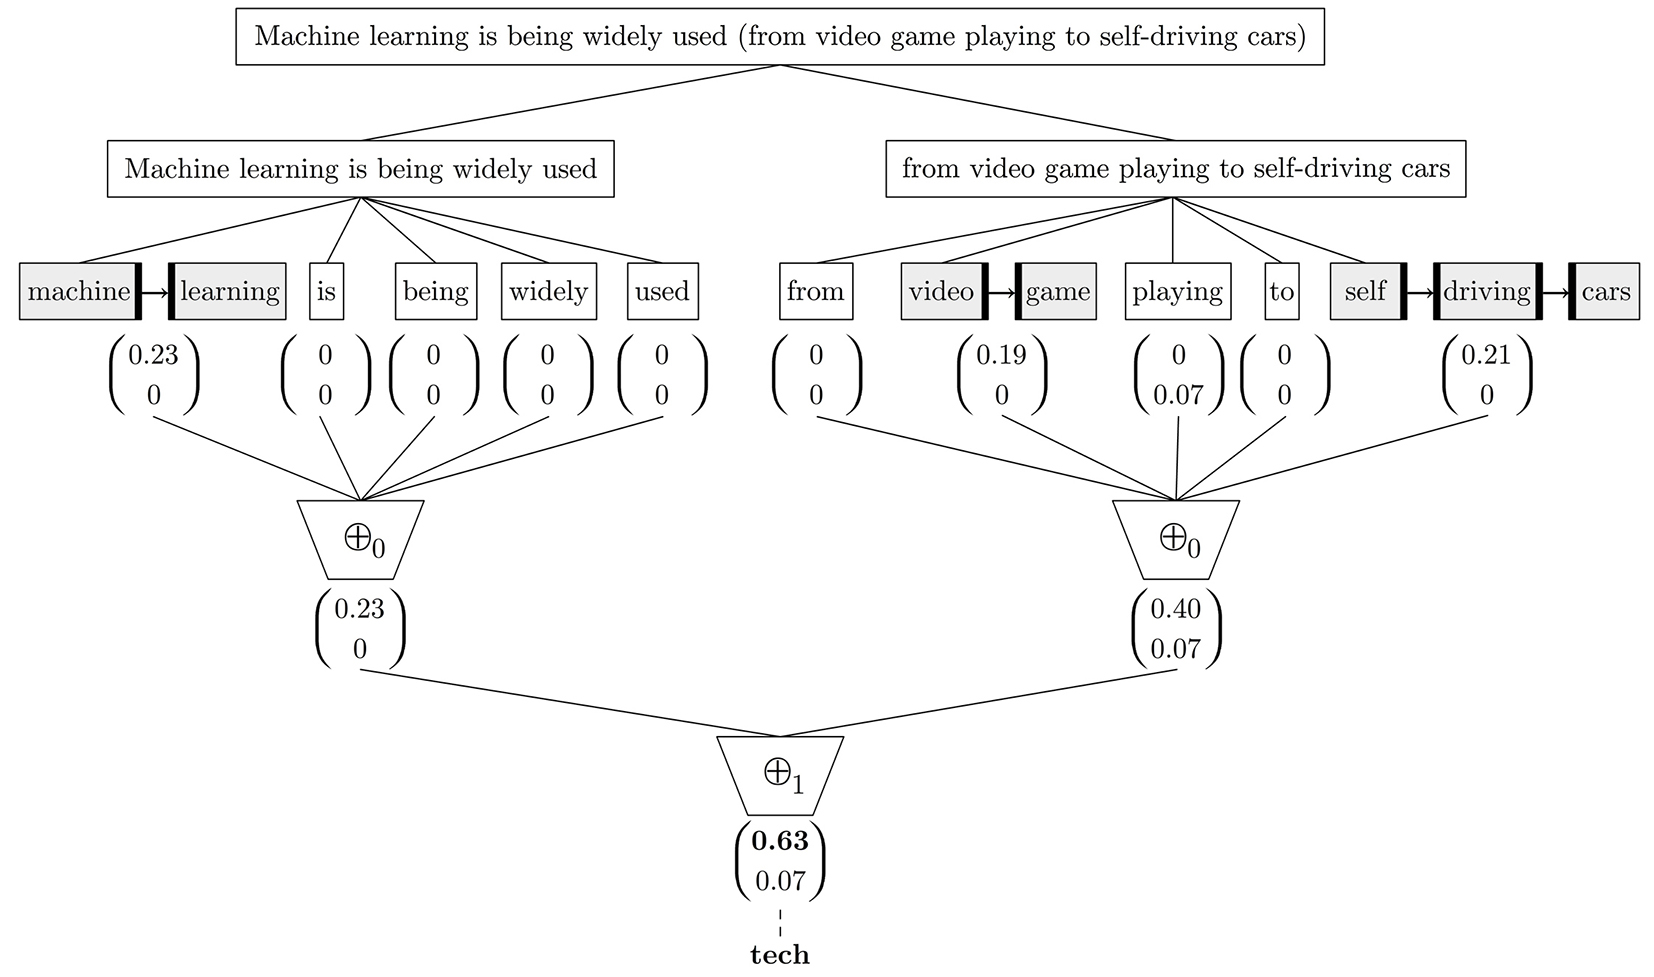
\includegraphics[width=190mm]{images/t-ss3-machine-learning}}
    \caption{
    Ejemplo de clasificación con $\tau$-SS3. Ya que SS3 ahora tiene la capacidad de valorar secuencias de palabras, esta vez fue capaz de clasificar correctamente la temática del documento como \emph{technology}.}
    % $\tau$-SS3 classification example. Since SS3 now has the ability to capture important word sequences, it is able to correctly classify the document's topic as $tech$.}
    \label{fig:t-ss3-example}
\end{figure*}


Luego, el ejemplo de clasificación incorrecta mostrado anteriormente en la \autoref{fig:ss3-example} podría clasificarse de forma correcta utilizando estos nuevos valores, como se ilustra en la \autoref{fig:t-ss3-example}.
En las siguiente sección, veremos cómo se podría implementar esta extensión formal en la práctica. Es decir, cómo podríamos implementar los algoritmos de aprendizaje y clasificación para, respectivamente, almacenar las secuencias aprendidas y reconocer estas secuencias importantes, dinámicamente, durante la clasificación.
% Then, the previously misclassified example could now be correctly classified, as shown in \autoref{fig:t-ss3-example}.
% In the following subsections, we will see how this formal extension is, in fact, implemented in practice. %, i.e., how the training and classification algorithms are implemented to store the learned sequences and to, in fact, dynamically recognize sequences like those of this example during classification time.


\subsection{Entrenamiento}


El algoritmo de aprendizaje original sólo necesitaba un diccionario de pares palabra-frecuencia por cada clase.
Luego, cada diccionario se actualizaba a medida que se procesaban nuevos documentos de entrenamiento, agregando nuevas palabras al diccionario y actualizando la frecuencia de las ya almacenadas.
Estas frecuencias eran el único elemento que se necesitaba guardar ya que era lo único necesario para calcular $lv(w,c)$.
% The original SS3 learning algorithm only needs a dictionary of term-frequency pairs for each category.
% Each dictionary is updated as new documents are processed ---i.e., unseen terms are added and frequencies of already seen terms are updated.
% Note that these frequencies are the only elements we need to store since to compute $lv(w,c)$ we only need to know $w$'s frequency in $c$, $tf_{w,c}$ (see \autoref{eq:lv}).

\begin{algorithm}[t]
\small
\caption{\small Nuevo algoritmo de aprendizaje. Redefinición de la función \textproc{Aprender-Documento} del \autoref{alg:training} original (véase página \pageref{alg:training}). Notar que aquí $texto$ es una secuencia de unidades léxicas que incluye no sólo palabras sino también signos de puntuación. $MAX\_NIVEL$ almacena el tamaño máximo permitido de secuencia.}
% Learning Algorithm. Note that $text$ is a sequence of lexical units (terms) which includes not only words but also punctuation marks.  $MAX\_NIVEL$ stores the maximum allowed sequence length.}
\label{alg:t-ss3-training}
\begin{algorithmic}[1]
\Statex
\Procedure{Aprender-Documento}{$texto$, \emph{etiqueta}}
	\State \Input $texto$, una secuencia de unidades léxicas del documento
	\State \inputindent \emph{etiqueta}, la etiqueta de la clase a la que pertenece el documento
	\State \LocalVariables $cursores$, un conjunto de nodos del árbol de prefijos
	\State
	\State \Call{Árbol-De-Prefijos}{} $\gets$ el árbol correspondiente a la clase dada por \emph{etiqueta}
	\State $cursores$ $\gets$ conjunto vacío
	\For{\emph{término} \In $texto$}
		\If{\emph{término} \textbf{no es} una palabra}
			\State $cursores$ $\gets$ conjunto vacío
		\Else
		    \State agregar \Call{Árbol-De-Prefijos}{}.\Call{Raíz}{} a $cursores$
		    \For{$nodo$ \In $cursores$}
		        \If{$nodo$ \textbf{no} tiene un hijo para \emph{término}}
		            \State $nodo$.\Call{Nodo-Hijo}{}.\Call{nuevo}{\emph{término}}
		        \EndIf
		        \State $nodo\_hijo$ $\gets$ $nodo$.\Call{Nodo-Hijo}{}[\emph{término}]
		        \State $nodo\_hijo$.\Call{Frecuencia}{} $\gets$ $nodo\_hijo$.\Call{Frecuencia}{} + 1
		        \If{$nodo\_hijo$.\Call{Nivel}{} $\ge$ $MAX\_NIVEL$}
		            \State remover $nodo$ de $cursores$
		        \Else
		            \State reemplazar $nodo$ con $nodo\_hijo$ en $cursores$
		        \EndIf
		    \EndFor
		\EndIf
	\EndFor
\EndProcedure
\end{algorithmic}
\end{algorithm}

Del mismo modo, el nuevo algoritmo de aprendizaje para $\tau$-SS3 sólo necesita almacenar las frecuencias de todas las secuencias de palabras observadas en los documentos de entrenamiento.
% Likewise, $\tau$-SS3 learning algorithm only needs to store frequencies of all word sequences seen while processing training documents.
Más precisamente, dado un entero positivo $n$, necesitamos almacenar la frecuencia de todos los $k$-gramas de palabras observados durante el entrenamiento, con $1 \leq k \leq n$ ---es decir, palabras individuales, bigramas, trigramas, y así.
% More precisely, given a fixed positive integer $n$, it must store information about all word $k$-grams seen during training, with $1 \leq k \leq n$ ---i.e., single words, bigrams, trigrams, etc.
Para llevar esto a cabo, el nuevo algoritmo, dado en \autoref{alg:t-ss3-training}, utiliza un \emph{árbol de prefijos}\footnote{A esta estructura de datos también se la conoce como \emph{trie}.} \cite{trie1960, crochemore2009trie} para almacenar todas las frecuencias.
% To achieve this, the new learning algorithm uses a \emph{prefix tree} (also called \emph{trie})\cite{trie1960, crochemore2009trie} to store all the frequencies, as shown in \autoref{alg:training}.
Notar que, en lugar de haber utilizado $k$ diferentes diccionarios por cada clase para almacenar los distintos $k$-gramas (\emph{e.g.} uno para palabras, otro para bigramas, otro para trigramas, y así), se ha decidido utilizar un único \emph{árbol de prefijos}, ya que todos los n-gramas siempre serán prefijos de los n-gramas más largos.\footnote{Por ejemplo, ``Don'' es prefijo de ``Don Quijote``, que a su vez es prefijo de ``Don Quijote de'', prefijo de ``Don Quijote de la'', que finalmente es prefijo de ``Don Quijote de la Mancha''.}
% Note that instead of having $k$ different dictionaries, one for each $k$-grams (e.g. one for words, one for bigrams, etc.) we have decided to use a single prefix tree since all n-grams will share common prefix with the shorter ones.
Además, en lugar de procesar el documento de entrada $k$ veces, nuevamente, una vez por cada tipo de $k$-gramas, se han decidido utilizar $k$ múltiples cursores sobre un mismo árbol. Estos cursores permiten que se puedan almacenar los distintos $k$-gramas, en simultáneo y de corrida, a medida que se va procesando la secuencia de entrada en flujo.
% Additionally, note that instead of processing the input document $k$ times, again one for each $k$-grams, we have decided to use multiple cursors to be able to simultaneously store all sequences allowing the input to be processed as a stream.
Finalmente, para no desperdiciar espacio de almacenamiento, notar que las líneas 8 y 9 del \autoref{alg:t-ss3-training} aseguran que sólo se tengan en cuenta n-gramas que, en principio, ``tengan sentido'', es decir, aquellos que estén formados solamente por palabras ---\emph{i.e.} que no tengan símbolos de puntuación en el medio.
% Finally, note that lines 8 and 9 of \autoref{alg:t-ss3-training} ensure that we are only taking into account n-grams that make sense, i.e., those composed only of words.
Todas estas observaciones previas, así como también la intuición del algoritmo, son ilustradas con un sencillo ejemplo en la \autoref{fig:t-ss3-training}.
% All these previous observations, as well as the algorithm intuition, are illustrated with an example in \autoref{fig:t-ss3-training}.
Este ejemplo asume que el entrenamiento recién  ha comenzado por primera vez, y que el primer documento a ser procesado es la pequeña oración \emph{``Mobile APIs, for mobile developers''} 
% This example assumes that the training has just begun for the first time and that the short sentence, \emph{``Mobile APIs, for mobile developers''}, is the first document to be processed.
---por lo que el árbol continuará creciendo luego, a medida que nuevos documentos de entrenamiento sean procesados.
% Note that this tree will continue to grow, later, as more documents are processed.

\begin{figure*}[t]
    \centering
    \centerline{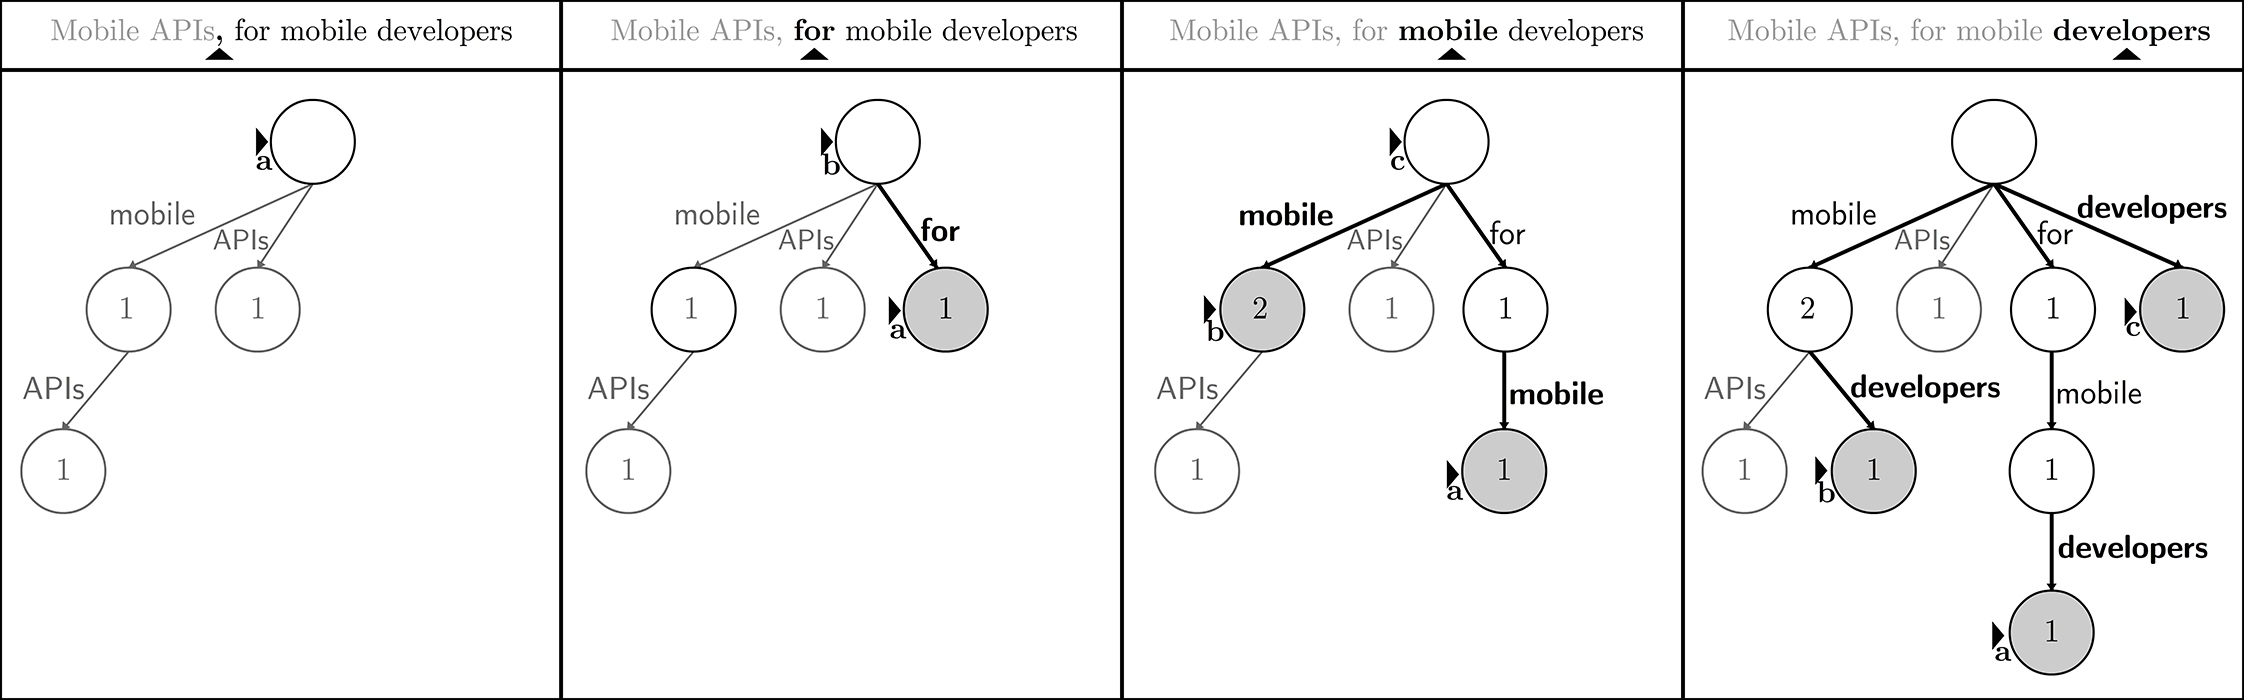
\includegraphics[width=190mm]{images/trie-training}}
    \caption{Ejemplo del proceso de entrenamiento. Las actualizaciones son indicadas con el color gris y la negrita.
    (a) las primeras dos palabras han sido consumidas y, por lo tanto, en el árbol se crearon tres nodos, uno para cada palabra y uno para el bigrama ``mobile APIs'', luego, en la entrada se encontró una coma, lo que provocó que se removieran todos los cursores y que se ubicara uno nuevo, $a$, apuntando a la raíz (véase líneas 9 y 10 del \autoref{alg:training});
    (b) se avanza una posición el cursor de entrada y se consume la palabra ``for'', se crea un nuevo nodo para esta palabra utilizando al cursor $a$ (véase línea 14), el cual luego se actualiza para apuntar a este nuevo nodo (línea 15 y 20) y un nuevo cursor $b$ es creado (línea 11) apuntando a la raíz;
    (c) se consume una nueva palabra desde la entrada, ``mobile'', usando el cursor $b$, se actualiza el nodo para esta palabra incrementando su frecuencia a 2 (línea 16). Además, un nuevo nodo es creado para el bigrama ``for mobile'' usando el antiguo cursor $a$ y, nuevamente, un nuevo cursor $c$ es creado para el nodo raíz (línea 11);
    (d) finalmente, se consume la palabra ``developers'' y, similarmente, nuevos nodos son creados para dicha palabra, el bigrama ``mobile developers'' y el trigrama ``for mobile developers''.}
    % Training example. Gray color and bold indicate an update.
    % (a) the first two words have been consumed and the tree has 3 nodes, one for each word and one for the bigram ``mobile APIs'', then a comma (,) is found in the input and \autoref{alg:training}'s line 9 and 10 have removed all the cursors and placed a new one, $a$, pointing to the root;
    % (b) the word ``for'' is consumed, a new node for this word is created using the node pointed by cursor $a$ (lines 14), $a$ is updated to point to this new node (line 15 and 20), the next term is read and a new cursor $b$ is created (line 11) in the root;
    % (c) ``mobile'' is consumed, using cursor $b$ the node for this word updated its frequency to 2 (line 16), a new node is created for the bigram ``for mobile'' using cursor $a$, and a new cursor $c$ is created in the root node (line 11);
    % (d) finally, the word ``developers'' is consumed and similarly, new nodes are created for word ``developers'', bigram ``mobile developers'' and trigram ``for mobile developers''.}
    \label{fig:t-ss3-training}
\end{figure*}

De esta forma, cada clase tendrá un \emph{árbol de prefijos} almacenando información relacionada a las distintas secuencias de palabras, habiendo así un nodo en el árbol por cada k-grama aprendido.
% Thus, each category has a \emph{prefix tree} storing information linked to word sequences in which there is a tree's node for each learned k-gram.
Notar que en el \autoref{alg:t-ss3-training}, nunca habrá más de $MAX\_NIVEL$ cursores y que, de igual manera, la altura de cada árbol nunca podrá ser mayor a $MAX\_NIVEL$, ya que los nodos del nivel 1 almacenarán unigramas, a nivel 2 bigramas, nivel 3 trigramas, y así sucesivamente.
% Note that in \autoref{alg:training}, there will never be more than $MAX\_LVL$ cursors and that the height of the trees will never grow higher than $MAX\_LVL$ since nodes at level 1 store 1-grams, at level 2 store 2-gram, and so on.
Finalmente, cabe destacar que este nuevo algoritmo de aprendizaje también nos permite conservar la principal virtud del original.
Esto es, el entrenamiento sigue siendo incremental\footnote{Es decir, el modelo sigue soportando \emph{online learning}.} ya que no hay necesidad de almacenar todos los documentos ni tener que reentrenar desde cero cada vez que se dispongan de nuevos documentos de entrenamiento, en su lugar, sólo será necesario actualizar los árboles ya existentes, creando nuevos nodos o actualizando las frecuencias.
% Finally, it is worth mentioning that this learning algorithm allows us to keep the original one's virtues. Namely, the training is still incremental (i.e., it supports online learning) since there is no need neither to store all documents nor to re-train from scratch every time new training documents are available, instead, it is only necessary to update the already created trees.
% Additionally, there is still no need to compute the document-term matrix because, during classification and using \autoref{eq:t-lv} and \autoref{eq:gv}, $gv$ could be dynamically computed based on the frequencies stored in the trees.

\subsection{Clasificación}

\begin{figure}[t!]
    \begin{subfigure}{0.5\textwidth}
        \centering
        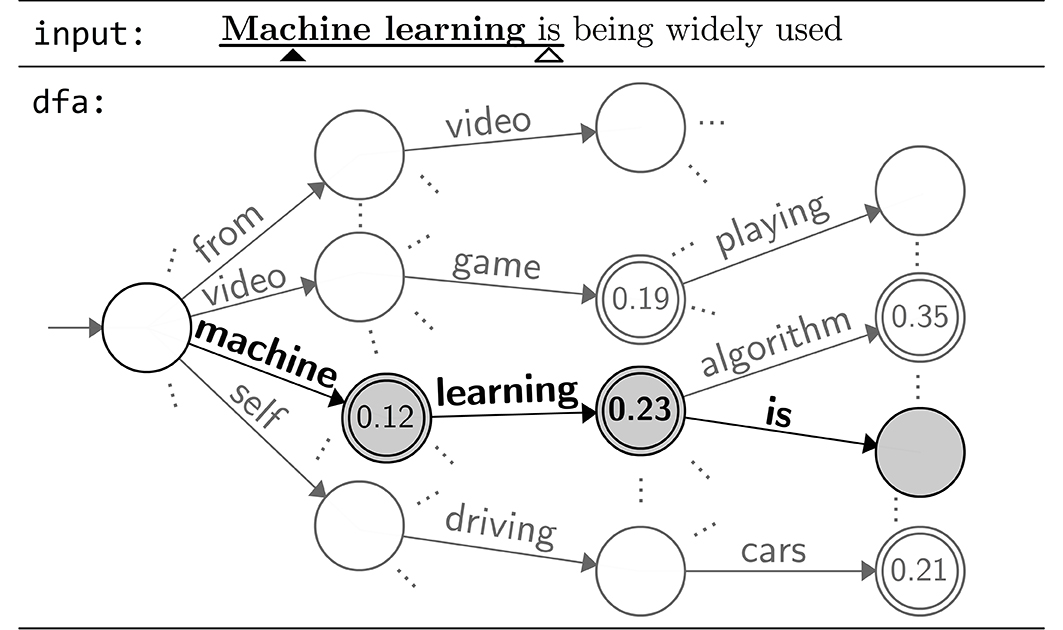
\includegraphics[width=\textwidth]{images/dfa0}
        \caption{}
        \label{fig:dfa_a}
    \end{subfigure}
    \begin{subfigure}{0.5\textwidth}
        \centering
        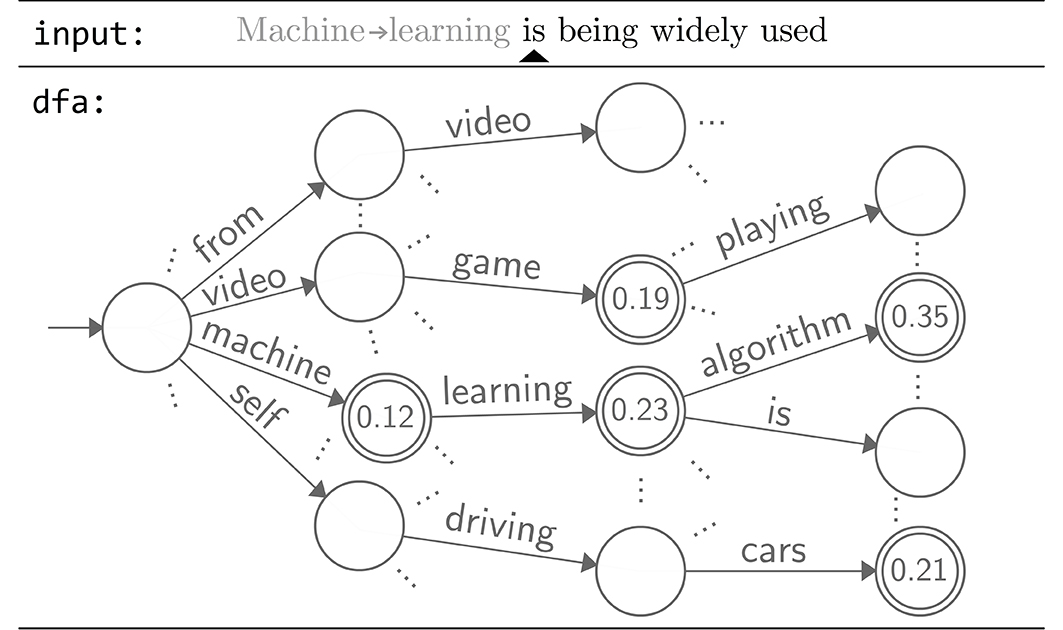
\includegraphics[width=\textwidth]{images/dfa1}
        \caption{}
        \label{fig:dfa_b}
    \end{subfigure}
\caption{Ejemplo de reconocimiento del mejor n-grama para la oración ``Machine learning is being widely used'', perteneciente al primer bloque oración del ejemplo de la \autoref{fig:t-ss3-example}.
% Example of recognizing the best n-gram for the first sentence block of \autoref{fig:t-ss3-example}, ``Machine learning is being widely used''.
Por simplicidad, en esta figura sólo se muestra el \ac{AFD} de \emph{technology}.
% For simplicity in this example, we only show the  \emph{technology}'s DFA.
Conceptualmente hay 2 cursores, uno negro ($\blacktriangle$) y uno blanco ($\vartriangle$). El primero, llamado ``cursor de entrada'', apunta al próximo término a ser consumido de la oración de entrada. El segundo, llamado ```cursor de búsqueda'', es el que se utiliza para alimentar a los autómatas con el fin de buscar/obtener el mejor n-grama. 
% There are conceptually 2 cursors, the black one ($\blacktriangle$) represents the input cursor and the white one ($\vartriangle$) the ``lookahead'' cursor to feed the automatons.
(a) El cursor de búsqueda ha avanzado alimentando al AFD con 3 palabras (``machine'', ``learning'', e ``is'') hasta que no hubo ninguna otra transición válida.
% (a) The lookahead cursor has advanced feeding the DFA with 3 words (``machine'', ``learning'', and ``is'') until no more state transitions were available.
En este punto, hay dos posibles estados finales, uno para ``machine'' y otro para ``machine learning'', seleccionándose este último por tener el mayor valor $gv$ (0.23);
% There were two possible final states, one for ``machine'' and another for ``machine$\rightarrow{}$learning'', the latter is selected since it has the highest $gv$ (0.23);
(b) Finalmente, luego de que el bigrama ``machine learning'' haya sido reconocido  y seleccionado, el cursor de entrada avanza 2 posiciones y está listo para comenzar el proceso de reconocimiento nuevamente, esta vez con ``is'' como la primer palabra para alimentar a los autómatas.}
% (b) Finally, after the bigram ``machine$\rightarrow{}$learning'' was recognized (see the first two word blocks painted in gray in \autoref{fig:t-ss3-example}), the input cursor advanced 2 positions and is ready to start the process again using ``is'' as the first word to feed the automatons.}
\label{fig:dfa}
\end{figure}

El nuevo algoritmo de clasificación será en gran medida el mismo que el original, dado en el \autoref{alg:classification} (véase página \pageref{alg:classification}), sólo será necesario cambiar el proceso por el cual las oraciones son divididas en palabras individuales, para permitir que sean divididas de forma más inteligente en secuencias de una o más palabras,
% The original classification algorithm will remain mostly unchanged\footnote{See Algorithm 1 from the original work \cite{burdisso2019}.}, we only need to change the process by which sentences are split into single words, by allowing them to be split into variable-length n-grams.
siendo estas secuencias ``las mejores posibles'' ---\emph{i.e.} las que tengan el máximo \emph{valor global}.
% Also, these n-grams must be ``the best possible ones'', i.e., having the maximum $gv$ value.
Para lograr este objetivo, utilizaremos el árbol de prefijos de cada clase para reconocer estas secuencias importantes como si fuera un \emph{\ac{AFD}}.
% To achieve this goal, we will use the prefix tree of each category as a \emph{deterministic finite automaton} (DFA) to recognize the most relevant sequences.
Esto es, virtualmente, cada nodo del árbol será considerado como un estado final del autómata siempre que su valor global\footnote{Más precisamente, el valor global del n-grama asociado a ese nodo.} sea mayor o igual que una constante pequeña dada, $\epsilon$.
% Virtually, every node will we considered as a final state if its $gv$ is greater or equal to a small constant $\epsilon$.
Así, al procesarse una oración, cada \ac{AFD} avanzará su cursor hasta que no pueda aplicar ninguna transición válida, luego, el n-grama asociado al estado final con el mayor valor global será el reconocido como ``la mejor secuencia de palabras''.
% Thus, every DFA will advance its input cursor until no valid transition could be applied, then the state (node) with the highest $gv$ value will be selected.
Para ayudar a visualizar este proceso, en la \autoref{fig:dfa} se lo ilustra con un sencillo ejemplo y en el \autoref{alg:t-ss3-classification} se brinda su algoritmo formal.
% This process is illustrated in more detail in \autoref{fig:dfa}.

\begin{algorithm}[t!]
\small
\caption{\small Algoritmo de clasificación a nivel oración.}
% \textproc{Map} aplica la función $gv$ a cada n-grama en $ngramas$ y devuelve una lista con los vectores resultantes.
% \textproc{Map} applies the $gv$ function to every n-gram in $ngramas$ and returns a list of resultant vectors.
% \textproc{Reduce} reduce $ngramas\_vcs$ a un único vector aplicando acumulativamente el operador $\oplus_{0}$.}
% \textproc{Reduce} reduces $ngramas\_vcs$ to a single vector by applying the $\oplus_{0}$ operator cumulatively.}
\label{alg:t-ss3-classification}
\begin{algorithmic}[1]
\Statex
\Function{Clasificar-Oración}{$texto$} \Returns un \emph{vector de confianza}
	\State \Input $texto$, la secuencia de unidades léxicas de la oración
	\State \LocalVariables $ngramas$, una secuencia de n-gramas de palabras
	\State \localvarsindent $ngramas\_vcs$, vectores de confianza
%  	\State
	\State $ngramas \gets$ \Call{Parsear}{$texto$}
	\State $ngramas\_vcs \gets$ \Call{Map}{}($gv$, $ngramas$)
	\State \Return \Call{Reduce}{}(\Call{$\oplus_{0}$}{}, $ngramas\_vcs$)
\EndFunction
\Statex \hrulefill
\Function{Parsear}{$texto$} \Returns una secuencia de n-gramas de palabras
    \State \Input $texto$, una secuencia de unidades léxicas
    % \State \GlobalVariables $categories$, las clases aprendidas
    \State \LocalVariables $mejor\_ngrama$, un n-grama
    \State \localvarsindent $resultado$, una secuencia de n-gramas
    \State \localvarsindent $mejores$, una lista de n-gramas
    % \State
    \State $cursor \gets$ el primer término de $texto$
    \While{$cursor$ \textbf{no es} vacío}
        \For{$clase$ \In $clases$}
            \State $mejores[clase] \gets$ \Call{Mejor-N-Grama}{$clase$, $cursor$}
        \EndFor
        \State $mejor\_ngrama \gets$ el n-grama con el mayor $gv$ de $mejores$
        \State agregar $mejor\_ngrama$ a $resultado$
        \State avanzar $cursor$ en $texto$ unas $mejor\_ngrama$.\Call{Longitud}{} posiciones
    \EndWhile
    \State \Return $resultado$
\EndFunction
\Statex \hrulefill
\Function{Mejor-N-Grama}{$clase$, \emph{término}} \Returns un n-grama
    \State \Input $clase$, una clase
    \State \inputindent \emph{término}, un cursor apuntando a un término en la oración
    \State \LocalVariables $estado$, un nodo del árbol de prefijos
    \State \localvarsindent $ngrama$, una secuencia de palabras
    \State \localvarsindent $mejor\_ngrama$, una secuencia de palabras
    % \State
    \State \Call{Árbol-De-Prefijos}{} $\gets$ el árbol asociado a la $clase$
    \State $estado \gets$ \Call{Árbol-De-Prefijos}{}.\Call{Raíz}{}
    \State agregar \emph{término} a $ngrama$
    \State $mejor\_ngrama \gets$ $ngrama$
    \While{$estado$ tenga un hijo para \emph{término}}
        \State $estado \gets$ $estado$.\Call{Nodo-Hijo}{}[\emph{término}]
        \State término $\gets$ próxima palabra en la oración
        \State agregar \emph{término} a $ngrama$
        \If{$gv(ngrama, clase) > gv(mejor\_ngrama, clase)$}
            \State $mejor\_ngrama \gets$ $ngrama$
        \EndIf
    \EndWhile
    \State \Return $mejor\_ngrama$
\EndFunction
\end{algorithmic}
\end{algorithm}

Finalmente, para que este proceso pueda ser incluido como parte del algoritmo de clasificación completo de SS3, sólo es necesario modificar la definición de \textproc{Clasificar-a-Nivel}$(texto, n)$ del algoritmo original (\autoref{alg:classification}), de forma tal que, cuando sea llamado con $n \leq 1$, llame a nuestra nueva función, \textproc{Clasificar-Oración}, dada en el \autoref{alg:t-ss3-classification}.
% Finalmente, el algoritmo formal se da en el \autoref{alg:t-ss3-classification}.\footnote{Notar que para que este algoritmo sea incluido como parte del algoritmo de clasificación original de SS3 (\autoref{alg:classification}), sólo necesitamos modificar la definición de \textproc{Clasificar-a-Nivel}$(texto, n)$ de forma tal que, cuando sea llamada con $n \leq 1$, llamará a nuestra nueva función, \textproc{Clasificar-oración}.}
% Finally, the formal algorithm is given in \autoref{alg:t-ss3-classification}.\footnote{Note that for this algorithm to be included as part of the SS3's overall classification algorithm, we only need to modify the definition of \textproc{Classify-At-Level}$(text, n)$ defined in Algorithm 1 of the original paper \cite{burdisso2019} so that, when called with $n \leq 1$, it will call our new function, \textproc{Classify-Sentence}.}
Notar que, de esta forma, en lugar de dividir las oraciones simplemente en palabras individuales, ahora se llamará a la función \textproc{Parsear} (véase  la línea 5),
% Note that instead of splitting the sentences into words simply by using a delimiter, now we are calling a \textproc{Parse} function on line 6.
la cual dividirá la oración ``inteligentemente'' en una lista de n-gramas de longitud variable.
% \textproc{Parse} intelligently splits the sentence into a list of variable length n-grams.
Siendo más precisos, la división se hará en base a la función \textproc{Mejor-N-Grama} (línea 18) que es la encargada de realizar, efectivamente, el proceso ilustrado en la \autoref{fig:dfa}, devolviendo el mejor n-grama para cada clase.
% This is done by calling the \textproc{Best-N-Gram} function on line 20 which carries out the process illustrated in \autoref{fig:dfa} to return the best n-gram for a given category.



\section{Evaluación Experimental}
\label{sec:tss3-results}

En esta sección se cubrirá el análisis experimental tanto de la extensión propuesta como del modelo original, abordando la detección anticipada de depresión, como en el capítulo anterior, más una nueva tarea, la detección anticipada de anorexia.
La siguiente subsección describe brevemente las tareas y los conjuntos de datos utilizados para entrenar y probar los modelos.
En la \autoref{sec:tss3-implementacion} se describen los detalles de implementación.
Finalmente, la \autoref{sec:tss3-result} examina los resultados obtenidos.

\subsection{Tareas y Conjunto de Datos}

La experimentación se condujo sobre tres tareas de detección anticipada de riesgos.
En particular, los modelos fueron evaluados, no sólo en la tarea del eRisk 2017 \cite{losada2017erisk} del capítulo anterior, sino también en dos nuevas tareas: detección anticipada de anorexia y detección anticipada de depresión del eRisk 2018 \cite{losada2018overview}.
% Así, demás como en el capítulo anterior detección anticipada de depresión tanto del eRisk 2017, como en el capítulo anterior, como del eRisk 2018 \cite{losada2017erisk, losada2018overview} y detección anticipada de anorexia eRisk 2018 \cite{losada2018overview}.
% Experiments were conducted on three of the CLEF's eRisk open tasks, namely eRisk 2017 and 2018 early depression detection \cite{losada2017erisk, losada2018overview} and eRisk 2018 early anorexia detection \cite{losada2018overview}.
Estas nuevas tareas también se centran en procesar secuencialmente el contenido publicado por usuarios de Reddit,
% These tasks focused on sequentially processing the content posted by users on Reddit.
por lo que, al igual que en el capítulo anterior, los conjuntos de datos que fueron utilizados en estas tareas consisten en colecciones de publicaciones creadas por un conjunto de usuarios de Reddit. %, los cuales aquí también volverán a referidos como ``sujetos''.
% Thus, the datasets that were used in these tasks are collections of writings (submissions) posted by a subset of Reddit users (referred to as ``subjects'').
Con el fin de comparar los resultados entre los diferentes modelos participantes, nuevamente, los conjuntos de datos fueron divididos en un conjunto fijo de entrenamiento y uno de prueba.
% In order to compare the results among different participants, as usual, each dataset is split into a training set and a test set.
Así, a los modelos se les entregó el conjunto de entrenamiento para entrenar y ajustar sus hiperparámetros antes de la etapa de prueba ---a cada equipo de investigación participante se le permitió utilizar hasta un máximo de cinco modelos distintos.
% Participating research teams were given the training set to train and tune their models offline and were allowed to submit up to five models each.
Para llevar a cabo la fase de prueba, los organizadores del eRisk decidieron, nuevamente, dividir el historial de publicaciones de cada usuario en diez bloques ---por lo que cada bloque contuvo el $10\%$ del historial completo del usuario.
% To carry out the test phase, eRisk organizers divided each user's writing history into 10 chunks.\footnote{Thus, each chunk contained 10\% of the complete user's history.}
Luego, durante la fase de prueba de clasificación anticipada, a los clasificadores se les dio el historial de publicaciones de cada usuario, un bloque a la vez, teniendo que decidir entre clasificar al usuario como positivo o, de lo contrario, esperar al siguiente bloque porque es requerida más información.
% Classifiers were given each user's history, one chunk at a time,
% % After receiving each chunk, classifiers were asked to decide which users were depressed/anorexic
% and after receiving each chunk, they could either classify the user as depressed/anorexic or wait for the next chunk.
% % Once a decision is emitted for a given user, it cannot be changed in later chunks.

Además, como es de esperarse, los modelos tuvieron que tomar la decisión correcta \emph{tan pronto como sea posible}, ya que la medida de evaluación utilizada fue nuevamente la medida \emph{ERDE} que, como sabemos del capítulo anterior, toma en cuenta no sólo la efectividad de la clasificación, sino también la demora en la toma de decisiones.
En particular, se volvieron a utilizar las medidas $ERDE_5$ y $ERDE_{50}$, las cuales toman como tiempo límite para las decisiones, respectivamente, la publicación número $5$ y $50$ de cada usuario.
% Furthermore, models had to make the correct decision \emph{as early as possible} since their performance was measured taking into account not only the effectiveness but also the delay of their decisions.
% Namely, the evaluation metric that was used is called \emph{Early Risk Detection Error} (ERDE).
% In our case, the performance of all participating models was measured using $ERDE_5$ and $ERDE_{50}$.


\subsection{Detalles de Implementación}
\label{sec:tss3-implementacion}
% \subsection{Implementation details}



La implementación de esta nueva versión del modelo fue codificada modificando la implementación original, realizada en el capítulo anterior, incorporándole la nueva versión de los algoritmos de entrenamiento y clasificación.
% La implementación también fue incorporada al paquete PyPI oficial de SS3, llamado PySS3\cite{burdisso2019pyss3}, el cual será introducido en el \autoref{cap:pyss3} y cuyo código fuente está disponible en Github  (\href{https://github.com/sergioburdisso/pyss3}{\url{https://github.com/sergioburdisso/pyss3}}).
% The new model implementation was coded in \emph{Python} using only built-in functions and data structures (such as \emph{dict}, \emph{map} and \emph{reduce} functions, etc.).
% The implementation was added to the official SS3's PyPI package, PySS3\cite{burdisso2019pyss3}, and its source code is available at \href{https://github.com/sergioburdisso/pyss3}{\url{https://github.com/sergioburdisso/pyss3}}.
Durante la experimentación, se fijó la longitud máxima de los n-gramas en $3$ (\emph{i.e.} se fijó $MAX\_LVL = 3$)\footnote{Se hicieron pruebas con diferentes valores, desde 2 hasta 10, pero el mejor desempeño se obtuvo con $MAX\_LVL = 3$.}
% We also fixed the maximum n-gram length to 3 (i.e., we set $MAX\_LVL = 3$).\footnote{We tried using different values, from 2 to 10, but the best performance was obtained with $MAX\_LVL = 3$.}
y, además, para evitar desperdiciar memoria al dejar que los árboles digitales crezcan innecesariamente por la incorporación de ruido, se ejecutó un procedimiento de ``poda de árbol'' cada millón de palabras procesadas durante el entrenamiento. La poda consistió simplemente en la eliminación de todos los nodos (n-gramas) con una frecuencia menor o igual a 10.
% During experimentation, in order to avoid wasting memory by letting the digital trees grow unnecessarily large, every million words a ``pruning'' procedure was executed in which all the nodes with a frequency less or equal than 10 were removed.

\begin{table}[t]
\centering
\caption{Resultados para la tarea de detección anticipada de depresión del eRisk 2017, ordenada por $ERDE_{50}$. Del total de 30 modelos que fueron enviados por los 8 equipos de investigación, aquí sólo se muestran los que obtuvieron el mejor $ERDE_{5}$ y el mejor $ERDE_{50}$ de cada equipo.}
% \caption{Results on the eRisk 2017 ``Early Depression Detection'' task ordered by ERDE$_{50}$ (the lower, the better). A total of 30 models were submitted by 8 research teams. Here we are only showing the model with best $ERDE_5$ and the model with the best $ERDE_{50}$ of each participating team.}
\label{tab:results-d2017}
\begin{tabular}{l | c c}
\hline
Modelo & $ERDE_{5}$ & $ERDE_{50}\blacktriangle$ \\ \hline
\textbf{$\tau$-SS3}$\star$ & \textbf{12.6\%} & \textbf{7.70\%}  \\
\textbf{SS3}$\star$ & \textbf{12.6\%} & 8.12\% \\
UNSLA & 13.66\% & 9.68\%  \\
FHDO-BCSGA & 12.82\% & 9.69\% \\
UArizonaD & 14.73\% & 10.23\% \\
FHDO-BCSGB & 12.70\% & 10.39\% \\
UArizonaB & 13.07\% & 11.63\% \\
UQAMD & 13.23\% & 11.98\% \\
GPLC & 14.06\% & 12.14\% \\
CHEPEA & 14.75\% & 12.26\% \\
LyRE & 13.74\% & 13.74\% \\
\hline
\end{tabular}
\end{table}

% \begin{table}[t]
% \centering
% \caption{Resultados para la tarea de detección anticipada de depresión del eRisk 2017. Del total de 30 modelos que fueron enviados por los 8 equipos de investigación, aquí sólo se muestran los que obtuvieron el mejor $ERDE_{5}$ y el mejor $ERDE_{50}$ de cada equipo.}
% \label{tab:results-d2017}
% \begin{tabular}{l@{}c || l@{}c}
% \hline
% & $ERDE_5\blacktriangle$ & & $ERDE_{50}\blacktriangle$\\ \hline

% \textbf{$\tau$-SS3}$\star$ & \textbf{12.60\%} & \textbf{$\tau$-SS3}$\star$ & \textbf{7.70\%} \\
% \textbf{SS3}$\star$ & \textbf{12.60\%} & \textbf{SS3}$\star$ & 8.12\% \\
% FHDO-BCSGB & 12.70\% & UNSLA & 9.68\%  \\
% FHDO-BCSGA & 12.82\% & FHDO-BCSGA & 9.69\% \\
% UArizonaB & 13.07\% & UArizonaD & 10.23\% \\
% UQAMD & 13.23\% & FHDO-BCSGB & 10.39\% \\
% UNSLA & 13.66\% & UArizonaB & 11.63\% \\
% LyRE & 13.74\% & UQAMD & 11.98\% \\
% GPLC & 14.06\% & GPLC & 12.14\% \\
% UArizonaD & 14.73\% & CHEPEA & 12.26\% \\
% CHEPEA & 14.75\% & LyRE & 13.74\% \\

% \hline
% \hline
% \end{tabular}
% \end{table}

Finalmente, dado que se quiere realizar una comparación directa y justa con el modelo original, se utilizaron los mismos valores de hiperparámetros que en el capítulo anterior.
% Finally, since we wanted to perform a direct (and fair) comparison against the original SS3 model, we decided to use the same hyperparameter values that were used in the SS3 original paper \cite{burdisso2019}.
Por lo tanto, se fijó $\lambda=\rho=1$ y $\sigma= 0.455$, los cuales, como vimos, habían sido originalmente seleccionados aplicando una búsqueda en grilla minimizando la medida $ERDE_{50}$ sobre el conjunto de entrenamiento, usando una \emph{validación cruzada de 4 iteraciones}.
% Therefore, we set $\lambda=\rho=1$ and $\sigma= 0.455$, which were originally selected by applying a grid search to minimize the $ERDE_{50}$ metric over the training data using 4-fold cross-validation.
Además, por los mismos motivos, como \emph{operadores de resumen}, $\oplus_j$, para todo nivel $j$, se volvió a utilizar la suma de vectores.
% Furthermore, as in the original work, vector addition was used as the \emph{summary operator}, $\oplus_j$, for all the levels.
Del mismo modo, se utilizó la misma política de clasificación anticipada, es decir, los usuarios se clasificaron como positivo tan pronto como el \emph{valor de confianza} positivo, acumulado hasta ese momento, fuese mayor que el negativo.
% Likewise, the same policy for early classification was also applied, i.e., users were classified as positive as soon as the positive accumulated \emph{confidence value} exceeded the negative one.
Finalmente, con respecto al preprocesamiento, no se utilizó ningún método especial salvo una simple normalización eliminando los acentos y convirtiendo el texto a minúsculas, al igual que en el capítulo anterior.\footnote{
Se probaron otros métodos como \emph{stemming} y \emph{lemmatization} utilizando el paquete \emph{Natural Language Toolkit} (NLTK) de Python, pero al contrario de lo que esperábamos inicialmente, el rendimiento del modelo se redujo.}
% Regarding preprocessing, as in the original work, no method was used except for simple accents removal, lowercase conversion, and tokenization.\footnote{
% We also tried performing stemming and lemmatization using the Natural Language Toolkit (NLTK), but contrary to what we initially expected, the early classification performance was reduced.
% }
Esta configuración experimental nos aseguró que, fuera de la adición de los nuevos n-gramas de palabras, ningún otro factor pudiera estar influyendo en los resultados obtenidos.



\subsection{Resultados Experimentales}
\label{sec:tss3-result}



\begin{table}[t]
\centering
\caption{Resultados para la tarea de detección anticipada de depresión del eRisk 2018, ordenada por $ERDE_{50}$. Del total de 44 modelos que fueron enviados por los 11 equipos de investigación, aquí sólo se muestran los que obtuvieron el mejor $ERDE_{5}$ y el mejor $ERDE_{50}$ de cada equipo.}
% \caption{Results on the eRisk 2018 ``Early Depression Detection'' task ordered by ERDE$_{50}$ (the lower, the better). A total of 44 models were submitted by 11 research teams. Here we are only showing the model with best $ERDE_5$ and the model with the best $ERDE_{50}$ of each participating team.}
\label{tab:results-d2018}
\begin{tabular}{l | c c}
\hline
Modelo & $ERDE_{5}$ & $ERDE_{50}\blacktriangle$ \\ \hline
\textbf{$\tau$-SS3}$\star$ & 9.48\% & \textbf{6.17\%} \\
\textbf{SS3}$\star$ & 9.54\% & 6.35\%  \\
FHDO-BCSGB & 9.50\% & 6.44\% \\
FHDO-BCSGA & 9.21\% & 6.68\% \\
LIIRB & 10.03\% & 7.09\% \\
PEIMEXC & 10.07\% & 7.35\% \\
UNSLA & \textbf{8.78\%} & 7.39\%  \\
LIIRA & 9.46\% & 7.56\% \\
UQAMA & 10.04\% & 7.85\% \\
LIRMMD & 11.32\% & 8.08\% \\
UDCA & 10.93\% & 8.27\% \\
UPFA & 10.01\% & 8.28\% \\
RKMVERID & 9.97\% & 8.63\% \\
UDCC & 9.47\% & 8.65\% \\
RKMVERIC & 9.81\% & 9.08\% \\
LIRMMA & 10.66\% & 9.16\% \\
TBSA & 10.81\% & 9.22\% \\
TUA1C & 10.86\% & 9.51\% \\
TUA1A & 10.19\% & 9.70\% \\
\hline
\end{tabular}
\end{table}

% SOLO SS3
% \begin{table}[t]
% \centering
% \caption{Resultados para la tarea de detección anticipada de depresión del eRisk 2018, ordenada por $ERDE_{50}$. Del total de 44 modelos que fueron enviados por los 11 equipos de investigación, aquí sólo se muestran los que obtuvieron el mejor $ERDE_{5}$ y el mejor $ERDE_{50}$ de cada equipo.}
% \label{tab:results-d2018}
% \begin{tabular}{l@{}c || l@{}c}
% \hline
% & $ERDE_5\blacktriangle$ & & $ERDE_{50}\blacktriangle$\\ \hline

% UNSLA & \textbf{8.78\%} & \textbf{SS3}$\star$ & \textbf{6.35\%}  \\
% FHDO-BCSGA & 9.21\% & FHDO-BCSGB & 6.44\% \\
% LIIRA & 9.46\% & FHDO-BCSGA & 6.68\% \\
% UDCC & 9.47\% & LIIRB & 7.09\% \\
% FHDO-BCSGB & 9.50\% & PEIMEXC & 7.35\% \\
% \textbf{SS3}$\star$ & 9.54\% & UNSLA & 7.39\%  \\
% RKMVERIC & 9.81\% & LIIRA & 7.56\% \\
% RKMVERID & 9.97\% & UQAMA & 7.85\% \\
% UPFA & 10.01\% & LIRMMD & 8.08\% \\
% LIIRB & 10.03\% & UDCA & 8.27\% \\
% UQAMA & 10.04\% & UPFA & 8.28\% \\
% PEIMEXC & 10.07\% & RKMVERID & 8.63\% \\
% TUA1A & 10.19\% & UDCC & 8.65\% \\
% LIRMMA & 10.66\% & RKMVERIC & 9.08\% \\
% TBSA & 10.81\% & LIRMMA & 9.16\% \\
% TUA1C & 10.86\% & TBSA & 9.22\% \\
% UDCA & 10.93\% & TUA1C & 9.51\% \\
% LIRMMD & 11.32\% & TUA1A & 9.70\% \\

% \hline
% \hline
% \end{tabular}
% \end{table}

% \begin{table}[t]
% \centering
% \caption{Resultados para la tarea de detección anticipada de depresión del eRisk 2018, ordenada por $ERDE_{50}$. Del total de 44 modelos que fueron enviados por los 11 equipos de investigación, aquí sólo se muestran los que obtuvieron el mejor $ERDE_{5}$ y el mejor $ERDE_{50}$ de cada equipo.}
% \label{tab:results-d2018}
% \begin{tabular}{l@{}c || l@{}c}
% \hline
% & $ERDE_5\blacktriangle$ & & $ERDE_{50}\blacktriangle$\\ \hline

% UNSLA & \textbf{8.78\%} & \textbf{$\tau$-SS3}$\star$ & \textbf{6.17\%} \\
% FHDO-BCSGA & 9.21\% & \textbf{SS3}$\star$ & 6.35\%  \\
% LIIRA & 9.46\% & FHDO-BCSGB & 6.44\% \\
% UDCC & 9.47\% & FHDO-BCSGA & 6.68\% \\
% \textbf{$\tau$-SS3}$\star$ & 9.48\% & LIIRB & 7.09\% \\
% FHDO-BCSGB & 9.50\% & PEIMEXC & 7.35\% \\
% \textbf{SS3}$\star$ & 9.54\% & UNSLA & 7.39\%  \\
% RKMVERIC & 9.81\% & LIIRA & 7.56\% \\
% RKMVERID & 9.97\% & UQAMA & 7.85\% \\
% UPFA & 10.01\% & LIRMMD & 8.08\% \\
% LIIRB & 10.03\% & UDCA & 8.27\% \\
% UQAMA & 10.04\% & UPFA & 8.28\% \\
% PEIMEXC & 10.07\% & RKMVERID & 8.63\% \\
% TUA1A & 10.19\% & UDCC & 8.65\% \\
% LIRMMA & 10.66\% & RKMVERIC & 9.08\% \\
% TBSA & 10.81\% & LIRMMA & 9.16\% \\
% TUA1C & 10.86\% & TBSA & 9.22\% \\
% UDCA & 10.93\% & TUA1C & 9.51\% \\
% LIRMMD & 11.32\% & TUA1A & 9.70\% \\

% \hline
% \hline
% \end{tabular}
% \end{table}

\begin{table}[t]
\centering
\caption{Resultados para la tarea de detección anticipada de anorexia del eRisk 2018, ordenada por $ERDE_{50}$. Del total de 34 modelos que fueron enviados por los 9 equipos de investigación, aquí sólo se muestran los que obtuvieron el mejor $ERDE_{5}$ y el mejor $ERDE_{50}$ de cada equipo.}
% \caption{Results on the eRisk 2018 ``Early Anorexia Detection'' task ordered by ERDE$_{50}$ (the lower, the better). A total of 34 models were submitted by 9 research teams. Here we are only showing the model with best $ERDE_5$ and the model with the best $ERDE_{50}$ of each participating team.}
\label{tab:results-a2018}
\begin{tabular}{l | c c}
\hline
Modelo & $ERDE_{5}$ & $ERDE_{50}\blacktriangle$ \\ \hline
FHDO-BCSGD & 12.15\% & \textbf{5.96\%}  \\
\textbf{$\tau$-SS3}$\star$ & \textbf{11.31\%} & 6.26\%  \\
FHDO-BCSGE & 11.98\% & 6.61\%  \\
\textbf{SS3}$\star$ & 11.56\% & 6.69\% \\
FHDO-BCSGB & 11.75\% & 6.84\%  \\
PEIMEXB & 12.41\% & 7.79\%  \\
UNSLB & 11.40\% & 7.82\%  \\
RKMVERIA & 12.17\% & 8.63\%  \\
LIIRB & 13.05\% & 10.33\%  \\
LIIRA & 12.78\% & 10.47\%  \\
TBSA & 13.65\% & 11.14\%  \\
UPFA & 13.18\% & 11.34\%  \\
UPFD & 12.93\% & 12.30\%  \\
TUA1C & 13.53\% & 12.57\%  \\
LIRMMB & 14.45\% & 12.62\%  \\
LIRMMA & 13.65\% & 13.04\%  \\
\hline
\end{tabular}
\end{table}

% \begin{table}[t]
% \centering
% \caption{Resultados para la tarea de detección anticipada de anorexia del eRisk 2018, ordenada por $ERDE_{50}$. Del total de 34 modelos que fueron enviados por los 9 equipos de investigación, aquí sólo se muestran los que obtuvieron el mejor $ERDE_{5}$ y el mejor $ERDE_{50}$ de cada equipo.}
% \label{tab:results-a2018}
% \begin{tabular}{l@{}c || l@{}c}
% \hline
% & $ERDE_5\blacktriangle$ & & $ERDE_{50}\blacktriangle$\\ \hline

% UNSLB & \textbf{11.40\%} & FHDO-BCSGD & \textbf{5.96\%} \\
% \textbf{SS3}$\star$ & 11.56\% & FHDO-BCSGE & 6.61\% \\
% FHDO-BCSGB & 11.75\% & \textbf{SS3}$\star$ & 6.69\% \\
% FHDO-BCSGE & 11.98\% & FHDO-BCSGB & 6.84\% \\
% FHDO-BCSGD & 12.15\% & PEIMEXB & 7.79\% \\
% RKMVERIA & 12.17\% & UNSLB & 7.82\% \\
% PEIMEXB & 12.41\% & RKMVERIA & 8.63\% \\
% LIIRA & 12.78\% & LIIRB & 10.33\% \\
% UPFD & 12.93\% & LIIRA & 10.47\% \\
% LIIRB & 13.05\% & TBSA & 11.14\% \\
% UPFA & 13.18\% & UPFA & 11.34\% \\
% TUA1C & 13.53\% & UPFD & 12.30\% \\
% TBSA & 13.65\% & TUA1C & 12.57\% \\
% LIRMMA & 13.65\% & LIRMMB & 12.62\% \\
% LIRMMB & 14.45\% & LIRMMA & 13.04\% \\

% \hline
% \hline
% \end{tabular}
% \end{table}

% \begin{table}[t]
% \centering
% \caption{Resultados para la tarea de detección anticipada de anorexia del eRisk 2018, ordenada por $ERDE_{50}$. Del total de 34 modelos que fueron enviados por los 9 equipos de investigación, aquí sólo se muestran los que obtuvieron el mejor $ERDE_{5}$ y el mejor $ERDE_{50}$ de cada equipo.}
% \label{tab:results-a2018}
% \begin{tabular}{l@{}c || l@{}c}
% \hline
% & $ERDE_5\blacktriangle$ & & $ERDE_{50}\blacktriangle$\\ \hline

% \textbf{$\tau$-SS3}$\star$ & \textbf{11.31\%} & FHDO-BCSGD & \textbf{5.96\%} \\
% UNSLB & 11.40\% & \textbf{$\tau$-SS3}$\star$ & 6.26\% \\
% \textbf{SS3}$\star$ & 11.56\% & FHDO-BCSGE & 6.61\% \\
% FHDO-BCSGB & 11.75\% & \textbf{SS3}$\star$ & 6.69\% \\
% FHDO-BCSGE & 11.98\% & FHDO-BCSGB & 6.84\% \\
% FHDO-BCSGD & 12.15\% & PEIMEXB & 7.79\% \\
% RKMVERIA & 12.17\% & UNSLB & 7.82\% \\
% PEIMEXB & 12.41\% & RKMVERIA & 8.63\% \\
% LIIRA & 12.78\% & LIIRB & 10.33\% \\
% UPFD & 12.93\% & LIIRA & 10.47\% \\
% LIIRB & 13.05\% & TBSA & 11.14\% \\
% UPFA & 13.18\% & UPFA & 11.34\% \\
% TUA1C & 13.53\% & UPFD & 12.30\% \\
% TBSA & 13.65\% & TUA1C & 12.57\% \\
% LIRMMA & 13.65\% & LIRMMB & 12.62\% \\
% LIRMMB & 14.45\% & LIRMMA & 13.04\% \\

% \hline
% \hline
% \end{tabular}
% \end{table}

Como se describe con más detalle en la descripción general de cada tarea~\cite{losada2017erisk, losada2018overview} y en las \emph{Working Notes} del CLEF,\footnote{Véase sección ``Early Risk Prediction on the Internet'' de las \emph{Working Notes} del CLEF 2017 (\url{http://ceur-ws.org/Vol-1866/}) y 2018 (\url{http://ceur-ws.org/Vol-2125/}).} entre estas tres tareas del eRisk participaron un total de 180 modelos, los cuales cubren una gran variedad de clasificadores que van desde modelos simples hasta avanzados utilizando enfoques de \emph{aprendizaje profundo}.
% As it is described in more detail in the overview of each task\cite{losada2017erisk, losada2018overview} and the CLEF Working Notes,\footnote{Section ``Early risk prediction on the Internet'' of the CLEF Working Notes for 2017 (\url{http://ceur-ws.org/Vol-1866/}) and 2018 (\url{http://ceur-ws.org/Vol-2125/}).} a total of 180 models were submitted to these three eRisk tasks, ranging from simple to more advanced deep learning models.
Por ejemplo, similar a lo examinado con más detalle el capítulo anterior para la tarea eRisk 2017, en la \autoref{sec:ADD}, algunos grupos de investigación utilizaron clasificadores simples como \ac{MNB}, \ac{RL} o \ac{SVM}, mientras que otros utilizaron métodos más avanzados, tales como diferentes tipos de Redes Neuronales Recurrentes con \emph{embeddings}, distintas arquitecturas de Redes Neuronales Convoluciones, modelos basados en grafos o incluso el ensamble de múltiples clasificadores.
% For instance, some research groups used simple classifiers such as Multinomial Naive Bayes, Logistic Regression, or Support Vector Machine (SVM) while others made use of more advanced methods such as different types of Recurrent Neural Networks with embeddings, graph-based models, or even ensemble of multiple classifiers.

\begin{figure*}[t!]
    \centering
    \begin{subfigure}{0.75\textwidth}
        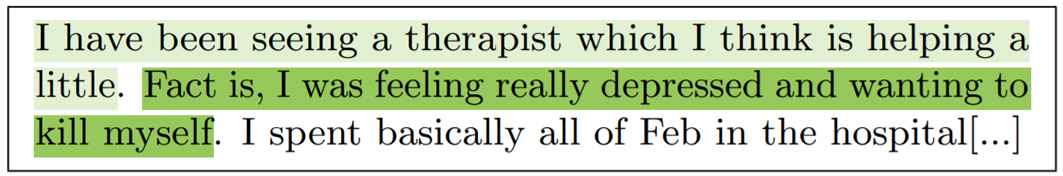
\includegraphics[width=\textwidth]{images/vd-example-a}
        \caption{Explicación a nivel de oración original, dada por SS3}
        \label{fig:subject9579_descriptive_a_tss3}
    \end{subfigure}
    \begin{subfigure}{0.75\textwidth}
        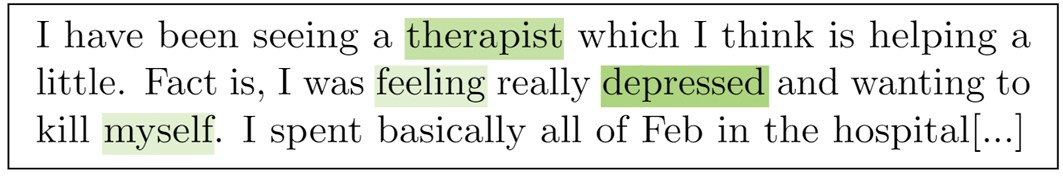
\includegraphics[width=\textwidth]{images/vd-example-c}
        \caption{Explicación a nivel de palabra original, dada por SS3}
        \label{fig:subject9579_descriptive_b_tss3}
    \end{subfigure}
    \begin{subfigure}{0.75\textwidth}
        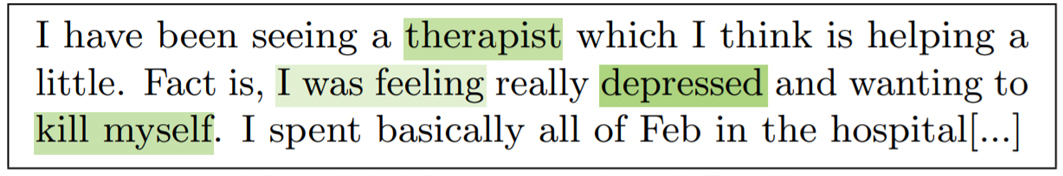
\includegraphics[width=\textwidth]{images/vd-example-b}
        \caption{Nueva explicación a nivel de palabra, dada por $\tau$-SS3}
        \label{fig:subject9579_descriptive_c_tss3}
    \end{subfigure}
\caption{Esta figura muestra un fragmento de la explicación visual dada al final del capítulo anterior. En particular, en (a) y (b) se vuelven a mostrar, respectivamente, las figuras (b) y (c) originales de la \autoref{fig:subject9579_descriptive}, en las que se muestra la publicación número 60 del sujeto 9579 de la tarea eRisk 2017, a dos niveles de explicación (a) oraciones y (b) palabras.
% Los bloques se pintan en relación a los verdaderos \emph{valores de confianza} obtenidos para la clase ``depresivo'' después de la experimentación.
% Esta explicación visual se muestra en dos niveles diferentes: (a) oraciones y (b) palabras.
Además, con fines comparativos, ahora se ha incluido en (c) la nueva explicación visual dada por $\tau$-SS3 para la misma publicación.
Notar que esta nueva explicación resalta información más rica, a saber, el trigrama ``I was feeling'' y el bigrama ``kill myself'', mejorando así la riqueza de las explicaciones visuales.}

% \caption{Esta figura muestra cómo se podría brindar una explicación visual del proceso de clasificación en la tarea abordada. Como mencionamos anteriormente, SS3 nos permite visualizar las razones detrás de la clasificación en diferentes niveles, en nuestro caso: (a) publicaciones, párrafos, (b) oraciones y/o (c) palabras. Cada uno de los segmentos está coloreado en relación al \emph{valor de confianza} positivo, real, obtenido en los experimentos realizados.}

% \caption{This figure shows a fragment of the visual explanation given by SS3 in Figure 9 of the original article \cite{burdisso2019}. It shows the subject 9579's writing 60 of the 2017 depression detection task. Blocks are painted proportionally to the true \emph{confidence values} obtained for the ``\emph{depressed}'' category after experimentation. This visual explanation is shown at two different levels: (a) sentences and (b) words. For comparison purposes, in (c), we now show the new visual explanation given by $\tau$-SS3. Note that more useful information is now shown, namely the trigram ``I was feeling'' and the bigram ``kill myself'', improving the richness of visual explanations.}
\label{fig:subject9579_descriptive_ts33}
\end{figure*}

Los resultados obtenidos para cada una de las tres tareas se muestran, respectivamente, en la \autoref{tab:results-d2017}, \autoref{tab:results-d2018} y \autoref{tab:results-a2018}.
% Results for each one of the three tasks are shown in \autoref{tab:results-d2017}, \autoref{tab:results-d2018}, and \autoref{tab:results-a2018}, respectively.
Como se puede observar, $\tau$-SS3 mejoró ligeramente el desempeño de SS3 en las tres tareas.
% As can be seen, although not significantly, $\tau$-SS3 improves SS3's performance in all three tasks.
Además, $\tau$-SS3 obtuvo los mejores valores de $ERDE_{50}$ para ambas tareas de detección de depresión. Sin embargo, en la tarea de detección de anorexia, obtuvo el segundo mejor valor, por debajo del modelo ``FHDO-BCSGD''~\cite{trotzek2018word}, el cual consiste en una Red Neuronal Convolucional con \emph{embeddings} de palabras obtenidos con \emph{fastText}.
% Furthermore, $\tau$-SS3 obtained the best $ERDE_{50}$ values in both depression detection tasks. However, it obtained the second-best value in the anorexia detection task; the best value was obtained by the FHDO-BCSGD\cite{trotzek2018word} model, which consists of a Convolutional Neural Network (CNN) with \emph{fastText} word embeddings.
En cuanto a $ERDE_{5}$, $\tau$-SS3 también superó a los otros modelos tanto en la tarea de detección de anorexia como en la de detección de depresión del año 2017.
Sin embargo, el mejor valor $ERDE_{5}$ en la tarea de detección de depresión del año 2018 lo obtuvo el modelo ``UNSLA''~\cite{funez2018}, que consiste en un clasificador \ac{SVM} que utiliza una representación de documento especial, denominada ``FTVT'', que tiene en cuenta el aspecto temporal al incorporar información relacionada al número de bloque siendo procesado en el momento.
Vale la pena mencionar que, aunque no se incluyen aquí, el nuevo modelo también mejoró el desempeño original de SS3 en términos de las medidas tradicionales, \emph{precision}, \emph{recall} y $F_1$.
% Regarding $ERDE_{5}$, $\tau$-SS3 also outperformed all the other models in both the anorexia detection and the 2018 depression detection tasks.
% However, the best value in the 2018 depression detection task was obtained by the UNSLA\cite{funez2018} model, which consists of an SVM classifier using a novel (time-aware) document representation, called FTVT.
% It is worth mentioning that, although not included in the tables, the new model also improved the original SS3's performance in terms of the standard (timeless) measures, precision, recall, and $F_1$.
Por ejemplo, en la tarea de detección anticipada de depresión abordada en el capítulo anterior, el \emph{recall}, \emph{precision} y $F_1$ de $\tau$-SS3 fueron $0.55$, $0.43$ y $0.77$, respectivamente, contra $0.52$, $0.44$ y $0.63$ de SS3.
% For instance, in the eRisk 2017 ``Early Depression Detection'' task, $\tau$-SS3's recall, precision and $F_1$ were 0.55, 0.43 and 0.77 respectively, against SS3's 0.52, 0.44 and 0.63.
Además, si bien estos valores no fueron los mejores entre todos los participantes, se situaron bastante por encima del promedio ($0.39$, $0.36$ y $0.51$), lo cual es considerablemente positivo teniendo en cuenta que los valores de hiperparámetros fueron seleccionados para optimizar la medida $ERDE_{50}$.
% Additionally, although these values were not the best among all participants, they were quite above the average (0.39, 0.36, and 0.51), which is not bad considering that our hyperparameter values were selected to optimize the $ERDE_{50}$ measure.

\section{Observaciones Finales}

\begin{table}[t]
\centering
\caption{Top 15 secuencias de una, dos y tres palabras ordenadas por \emph{valor global}, obtenidos para la tarea de detección anticipada de depresión del eRisk 2018.}
\label{tab:ngramas}
\begin{tabular}{l | l | l}
\hline
Unigramas & Bigramas & Trigramas \\ \hline
$depression$ & $my{\rightarrow}boyfriend$ & $i{\rightarrow}m{\rightarrow}feeling$ \\
$anxiety$ & $my{\rightarrow}skin$ & $cerave{\rightarrow}in{\rightarrow}the$ \\
$boyfriend$ & $my{\rightarrow}depression$ & $depression{\rightarrow}and{\rightarrow}anxiety$ \\
$depressed$ & $depression{\rightarrow}and$ & $i{\rightarrow}was{\rightarrow}diagnosed$ \\
$acne$ & $with{\rightarrow}depression$ & $was{\rightarrow}diagnosed{\rightarrow}with$ \\
$meds$ & $anxiety{\rightarrow}and$ & $anxiety{\rightarrow}and{\rightarrow}depression$ \\
$keto$ & $my{\rightarrow}husband$ & $my{\rightarrow}husband{\rightarrow}and$ \\
$cerave$ & $depression{\rightarrow}is$ & $husband{\rightarrow}and{\rightarrow}i$ \\
$makeup$ & $my{\rightarrow}anxiety$ & $a{\rightarrow}panic{\rightarrow}attack$ \\
$routine$ & $my{\rightarrow}pain$ & $my{\rightarrow}boyfriend{\rightarrow}and$ \\
$therapist$ & $panic{\rightarrow}attacks$ & $cerave{\rightarrow}foaming{\rightarrow}cleanser$ \\
$panic$ & $of{\rightarrow}depression$ & $i{\rightarrow}was{\rightarrow}feeling$ \\
$medication$ & $and{\rightarrow}depression$ & $an{\rightarrow}appointment{\rightarrow}with$ \\
$lotion$ & $and{\rightarrow}anxiety$ & $myself{\rightarrow}that{\rightarrow}i$ \\
$nyx$ & $pain{\rightarrow}and$ & $in{\rightarrow}the{\rightarrow}mood$ \\
\hline
\end{tabular}
\end{table}

En este capítulo introdujimos a $\tau$-SS3, una extensión del modelo original presentado en el capítulo anterior. Esta extensión le permite al modelo aprender a reconocer n-gramas de palabras de longitud variable ``sobre la marcha'', a medida que se procesa el texto de entrada ---en otras palabras, esta extensión le brinda al modelo la capacidad de reconocer patrones útiles sobre secuencias de texto.
Vimos que esta extensión fue llevada a la práctica utilizando, por cada categoría, un \emph{árbol de prefijos} para almacenar los n-gramas de longitud variable que se observan durante el entrenamiento y luego, durante la clasificación, esta misma estructura de datos es utilizada como un \emph{autómata finito determinista} que reconoce las secuencias de palabras importantes a medida que se consume la entrada.
Los resultados experimentales mostraron que $\tau$-SS3 superó levemente a SS3 tanto en términos de las medidas de desempeño tradicionales como en las medidas $ERDE_5$ y $ERDE_{50}$, lo que sugiere que los n-gramas aprendidos podrían, en efecto, contribuir positivamente al rendimiento del modelo.
Tal vez una de las causas de esta mejora se deba a que los n-gramas aprendidos, como se ilustra en la \autoref{tab:ngramas}, provocan que palabras previamente ignoradas de forma individual cobren importancia al ser consideradas junto a otras, como es el caso de las palabras ``my'' y ``I'' que predominan en los bigramas y trigramas aprendidos, reflejando el hecho de que el uso de la primera persona es relevante para este tipo de tareas.
Además, y quizás más importante, los n-gramas aprendidos también contribuyen a mejorar la expresividad de las explicaciones visuales dadas por el modelo, como se ilustra en la \autoref{fig:subject9579_descriptive_ts33}.\footnote{Las demos en vivo disponibles en línea (\href{http://tworld.io/ss3}{\url{http://tworld.io/ss3}}), mencionadas en el capítulo anterior, en realidad fueron implementadas utilizando a $\tau$-SS3, por lo que estas demos son capaces de reconocer secuencias de palabras importantes y resaltarlas en las explicaciones visuales dadas a los usuarios.}
La investigación futura debería centrarse en evaluar y analizar el espacio y la complejidad computacional de los algoritmos y estructuras de datos utilizados para implementar esta extensión del modelo original.
Además, sería interesante poder evaluar esta extensión en una mayor variedad de tareas para poder concluir con mayor solidez que, efectivamente, es superior al modelo original.
\hfill$\square$


% \section{Conclusiones y Trabajo Futuro}
% \label{sec:tss3-conclusion}

